% !TeX root = ../main.tex

\section{Approach}
\subsection{Architecture}
\begin{frame}{\insertsubsection}
	\only<1>{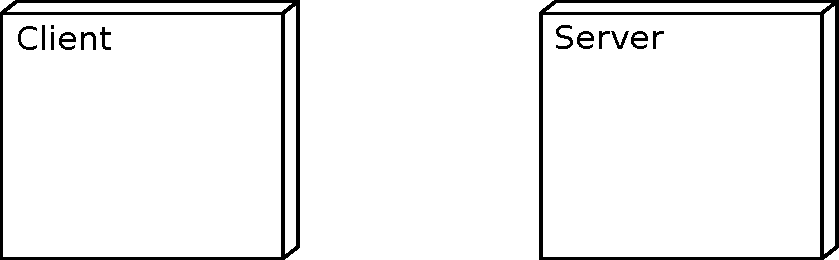
\includegraphics[width=\linewidth]{fig/architecture_overview_client_server.pdf}}
	\only<2>{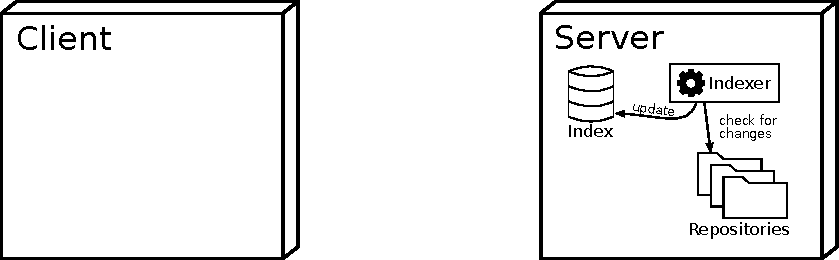
\includegraphics[width=\linewidth]{fig/architecture_overview_server.pdf}}
\end{frame}

\subsection{Index Creation}
\subsubsection{Normalization}
\begin{frame}{\insertsubsection}{\insertsubsubsection}
	\begin{center}
		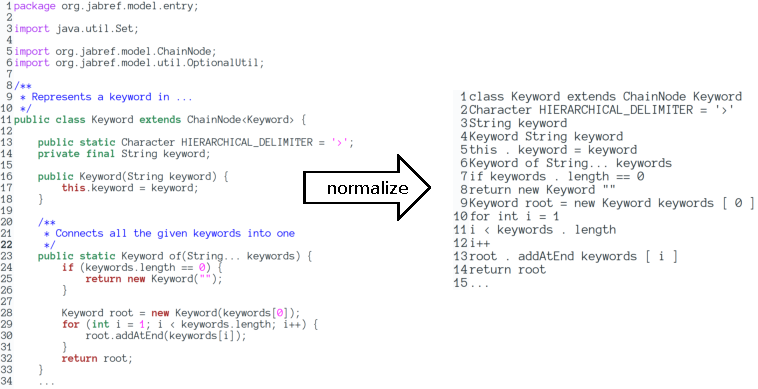
\includegraphics[width=0.9\linewidth]{fig/normalization_1.pdf}
	\end{center}
	\begin{itemize}
		\small
		\item Removes formatting, comments, access modifiers, brackets, import statements, ...
		\item Focus on features and properties relevant for comparing copied code
	\end{itemize}
\end{frame}

\subsubsection{Hashing chunks}
\begin{frame}{\insertsubsection}{\insertsubsubsection}
	\begin{center}
		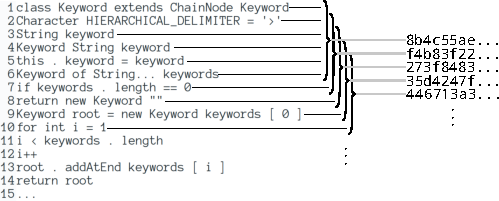
\includegraphics[width=0.9\linewidth]{fig/normalization_2.pdf}
	\end{center}
	\begin{itemize}
		\item Splitting normalized code into statements
		\item Group into chunks of 5 statements
		\item Location of chunk is stored in index
		\item Hash is used as key
	\end{itemize}
\end{frame}

\subsubsection{History Analysis}
\begin{frame}{\insertsubsection}{\insertsubsubsection}
	\begin{center}
		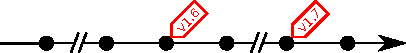
\includegraphics[width=\linewidth]{fig/history_analysis.pdf}
	\end{center}
	
	\begin{itemize}
		\item Analyzing history relevant to find old versions of a file
		\item Using git tags as reference points
		\item Re-indexing changed files between two versions
	\end{itemize}
\end{frame}

\subsection{Searching for Copied Code}
\begin{frame}{\insertsubsection}
	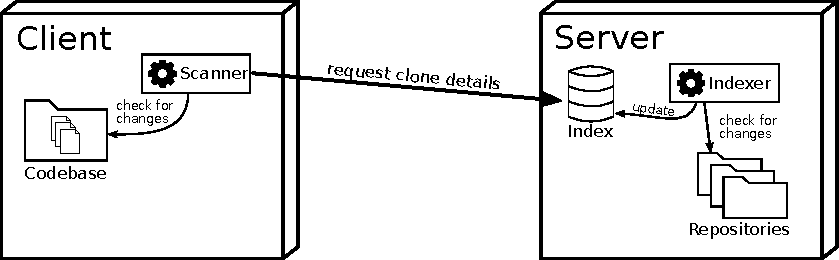
\includegraphics[width=\linewidth]{fig/architecture_overview_search.pdf}
\end{frame}

\subsubsection{Hash Filter}
\begin{frame}{\insertsubsection}{\insertsubsubsection}
	\textbf{Problem:} Lots of request have to be sent to server\\
	\pause
	\vspace{2mm}
	\textbf{Solution:} Bloom filter on client side
	\vspace{2mm}
	\begin{itemize}
		\small
		\item Data structure, calculated on server, downloaded to client
		\item Fraction in size compared to the index database\\ (37 GB $\rightarrow$ 200 MB)
		\item Client can decide whether a hash is part of the index with very small false positive probability (0,01\%)
		\item Reduces number of requests to a fraction
	\end{itemize}
\end{frame}

\begin{frame}{\insertsubsection}{Hash Filter in Use}
	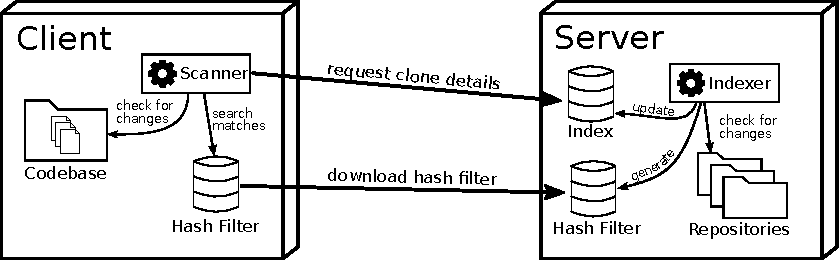
\includegraphics[width=\linewidth]{../written/figures/architecture_overview.pdf}
\end{frame}

%\begin{frame}{\insertsubsection}
%	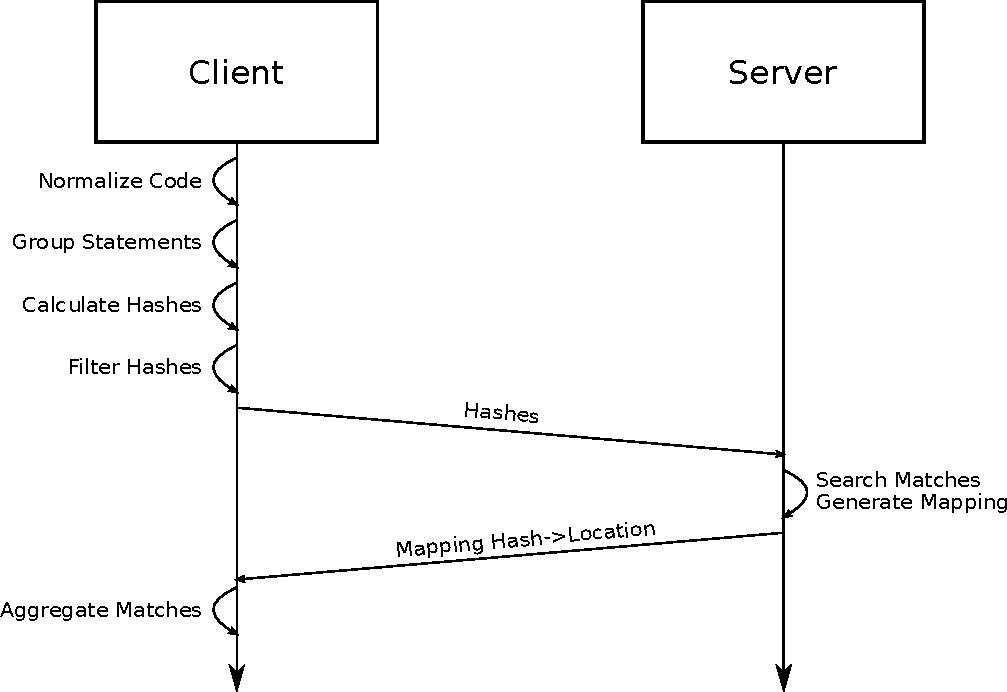
\includegraphics[width=\linewidth]{../written/figures/searching_copied_code.pdf}
%	
%	\pnote{
%		\begin{itemize}
%			\item ablauf suche
%			\item Download datenstruktur für bloom filter
%			\item normalize, group statements to chunks, hash
%			\item Filter hashes mit bloom filter
%			\item Details für übrige hashes anfragen
%			\item Server gibt für jeden hash locations zurück
%			\item Treffer auf client aggregiert und ausgewertet
%		\end{itemize}
%	}
%\end{frame}
